\documentclass[]{article}
\usepackage{amsmath}
\usepackage{graphicx}
%opening
\title{Gene network simulation in EuGENia Live}
\author{Joost van Pinxten}

\begin{document}

\maketitle

\section{Network description}
A gene network is an interaction network between different types of molecules. We will look at the (high-level) interactions inside a single cell. From our point of view, only the current amount of molecules and the rate of interaction between them is of interest. We can then model the gene network as a set of differential equations, leading to a (potentially) dynamical system (e.g. non-linear differential equations). Such dynamical systems cannot be always be analyzed mathematically, and the tool will support us with some simulation.

\subsection{Gene network palette}

As described before, there are several (types of) molecules in play; we have identified:

\begin{itemize}
	\item DNA: a static number of DNA-strands (molecules) inside a cell (typically 2)
	\item RNA: a dynamic number of (messenger) RNA, produced from the DNA-strands of interest
	\item Protein (or genes): a dynamic number of target protein, created from RNA molecules
\end{itemize}

We consider the 'chemical concentration' as the absolute number of molecules inside a cell; we do not normalize per volume, as the volume is equal for all concentrations. We can then define a production, consumption and degradation as follows;

\begin{itemize}
	\item produce: production per second = reaction rate * source molecule concentration
	\item degrade: degradation per second = reaction rate * source molecule concentration
	\item inhibit: description todo
	\item stimulate: description todo
\end{itemize}

\section{Example network}
For example, take the example network in Figure \ref{fig:example_1}; it is a very simple example where two DNA-strands produce a certain kind of RNA (at a specified reaction rate). This DNA degrades due to environmental circumstances and produces some kind of protein.

Define $N_{DNA}(t)$, $N_{RNA}(t)$, $N_{protein}(t)$ as the number of respective molecules (varying over time). With the RNA production $k_1$ and degradation rate $k_2$ and protein production  $k_3$ and degradation $k_4$ rate respectively, we can write the network from Figure 1 \ref{fig:example_1} in Newtonian notation as: 

\begin{equation}
\dot{N}_{RNA}(t) = k_1 \cdot N_{DNA}(t) - k_2 \cdot N_{RNA})(t)
\end{equation}

\begin{equation}
\dot{N}_{protein}(t) = k_3 \cdot N_{RNA}(t) - k_4 \cdot N_{protein}(t)
\end{equation}

Now, given initial conditions for $t=0$ for the concentrations, we can gain some insight into how far the concentrations may grow.

\begin{equation}
    N_{DNA}(t)= 
\begin{cases}
    2,& \text{if } t\geq 0\\
    0,              & \text{otherwise}
\end{cases}
\end{equation}
\begin{equation}
N_{RNA}(0) = 0
\end{equation}
\begin{equation}
N_{protein}(0) = 0
\end{equation}

This means that at $t=0$:

\begin{equation}
	\begin{aligned}
	\dot{N}_{RNA}(0) &= k_1 \cdot N_{DNA}(0) - k_2 \cdot N_{RNA}(0)\\
	&= k_1 \cdot 2 - k_2 \cdot 0\\
	&= 2 k_1 \\
	\dot{N}_{protein}(0)& = k_3 \cdot N_{RNA}(0) - k_4 \cdot N_{protein}(0)\\
	&= k_3 \cdot 0 - k_4 \cdot 0 \\
	&= 0
	\end{aligned}
\end{equation}

\begin{equation}
	\begin{aligned}
	\dot{N}_{protein}(0)& = k_3 \cdot N_{RNA}(0) - k_4 \cdot N_{protein}(0)\\
	&= k_3 \cdot 0 - k_4 \cdot 0 \\
	&= 0
	\end{aligned}
\end{equation}

The RNA concentration stabilizes ($t \geq 0$) when:
\begin{equation}
	\begin{aligned}
	\dot{N}_{RNA}(t)& = 0 \\
		\implies
	k_1 \cdot 2 - k_2 \cdot N_{RNA}(t) &= 0\\
		\implies
	N_{RNA}(t) &= \frac{2 k_1}{k_2} \\		
	\end{aligned}
\end{equation}

(You could even find out the time it takes to get near this point, by solving the differential equation into it's exponential function)

This is all \emph{approximated} by the simulation model. In our example; $k_1=0.06$, and $k_2= 0.006$. This means that $N_{RNA}(t_s)=20$ at some point.

The same goes for the protein; but this is also dependent on the (non-constant) $N_{RNA}(t)$, which means we can only approximate it by taking the highest $N_{RNA}(t)$ (this only works because it is a simple model). We then write:

\begin{equation}
	\begin{aligned}
	\dot{N}_{protein}(t)& = 0 \\
		\implies
	k_3 \cdot N{RNA}(t) - k_4 \cdot N_{protein}(t) &= 0\\
		\implies
	N_{protein}(t) &= \frac{\frac{2 k_1}{k_2}\cdot k_3}{k_4} \\		
	\end{aligned}
\end{equation}

With $k_3=0.04$ and $k_4=0.002$, this becomes $\frac{20 \cdot 0.04}{0.002} = 400$.

\begin{figure}
\label{fig:example_1}
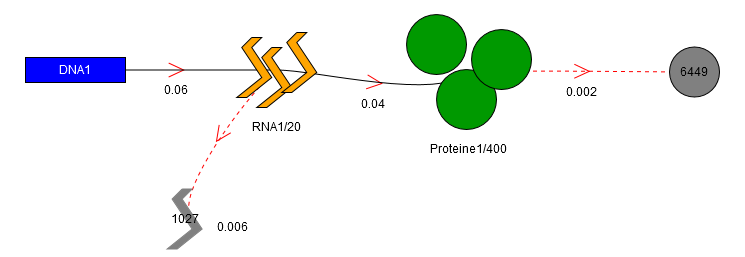
\includegraphics[width=\textwidth]{example1}
\caption{Example of a simple gene production network}
\end{figure}

\end{document}
